\section{Introduction}
\label{sec:intro}

Type 1 diabetes requires people to manage their blood glucose themselves, every day, with insulin. Too little insulin leads to hyperglycemia, conventionally glucose above 180 mg/dL, which over years damages the eyes, kidneys, nerves and blood vessels. Too much insulin leads to hypoglycemia, glucose below 70 mg/dL, which can cause confusion, seizures and loss of consciousness and can become dangerous quickly \parencite{battelino2019tir}. Continuous glucose monitors (CGM) measure glucose every five minutes, and that stream of readings makes it possible to forecast where glucose is heading. A forecast 60 minutes ahead is long enough to act on: there is time to eat carbohydrates before a low, or to correct a high with insulin.

A forecast is never exact, so its usefulness depends on how much it can be trusted. A prediction interval, called a band in this paper, gives a range that should contain the true future value with a stated probability. An 80\% band is honest, or calibrated, if the true value falls inside it 80\% of the time. A band that is too narrow gives false confidence: a person may skip a snack because the band says glucose will stay in range, and then go low. A band that is too wide triggers needless alarms and is soon ignored. Recent glucose forecasters increasingly report bands, using quantile outputs, mixture densities, Monte Carlo dropout, evidential layers or conformal methods \parencite[e.g.,][]{sergazinov2023gluformer}.

These bands are almost always evaluated by marginal coverage, the share of true values inside the band across all forecasts pooled together. Clinical use, however, is conditional. The cost of a miss depends on the situation: a forecast made at 110 mg/dL while glucose is falling fast matters far more than one made at 200 mg/dL while glucose is steady. A band can reach 80\% coverage on average while covering much less in the situations that matter most, because over-coverage elsewhere hides the shortfall. In the same way, a band can be honest for the average patient but not for a particular person, or honest across a month but not on a given day.

This paper asks whether a band around a forecast of glucose 60 minutes ahead stays honest where it is used: in each situation, for each patient, and on each day. A situation describes the moment the forecast is made. It combines the current glucose level with how much glucose changed over the previous 30 minutes, for example ``between 70 and 120 mg/dL and rising fast.'' Table~\ref{tab:situations} gives the exact cutoffs: five level ranges and five trend categories, which together give 25 situations. This paper addresses the first of the three questions, consistency across situations.

\begin{table}[htbp]
\caption{Glucose Levels and Trends That Define a Situation}
\label{tab:situations}
\small
\begin{tabular}{ll}
\hline
Level (current CGM reading) & Range \\
\hline
Low (hypoglycemia) & below 70 mg/dL \\
Low normal & 70 to 120 mg/dL \\
High normal & 120 to 180 mg/dL \\
High & 180 to 250 mg/dL \\
Very high & 250 mg/dL and above \\
\hline
Trend (change over the last 30 minutes) & Change \\
\hline
Falling fast & fell by more than 30 mg/dL \\
Falling slowly & fell by 10 to 30 mg/dL \\
Flat & changed by less than 10 mg/dL either way \\
Rising slowly & rose by 10 to 30 mg/dL \\
Rising fast & rose by 30 mg/dL or more \\
\hline
\end{tabular}

\vspace{2pt}
\noindent\textit{Note.} Each level range includes its lower edge. A situation is one level combined with one trend, so there are $5 \times 5 = 25$ situations.
\end{table}

The paper makes three contributions. First, it describes a large evaluation setting: per-patient forecasters for 215 people with type 1 diabetes from 11 public datasets. Three of the datasets were used to design the methods, and the other eight, with 153 patients, were held out and used only to test them. Second, it compares a standard band from financial econometrics, GARCH \parencite{bollerslev1986garch}, with a situation-aware band that learns a separate width for each situation, a form of group-conditional (Mondrian) conformal prediction \parencite{vovk2005alrw}. Third, it reports initial evidence that the situation-aware band is more consistent across situations than the standard band, including on the held-out datasets.

The paper is organized as follows. The Related Work section reviews glucose forecasting, uncertainty for glucose forecasts and conformal prediction. The Data section describes the 11 datasets and how patients and records were selected. The Methods section describes the forecaster, the situations, the bands and the measure of consistency. The Results section presents the initial results on consistency across situations, and the Discussion briefly interprets them. \todo{Analyses by patient and by day will follow in later versions.}

\section{Related Work}
\label{sec:related}

\textit{Glucose forecasting.} Short-term glucose forecasting from CGM, insulin and carbohydrate records is an active field, and most work aims at better point accuracy. Recent frameworks such as GLIMMER change how forecasters are trained so that errors in dangerous glucose ranges count more \parencite{glimmer2026}. Public datasets, including OhioT1DM \parencite{marling2020ohio}, AZT1D \parencite{azt1d2025} and the MetaboNet consolidation of many public datasets \parencite{metabonet2026}, now make it possible to test methods across many patients and settings.

\textit{Uncertainty for glucose forecasts.} A smaller body of work adds bands to glucose forecasts. Gluformer produces a predictive distribution from a transformer \parencite{sergazinov2023gluformer}. A Temporal Fusion Transformer study predicts the 10th, 50th and 90th percentiles of glucose 60 minutes ahead, which gives an 80\% band \parencite{rodriguezalmeida2025tft}, and another study compares Monte Carlo dropout with evidential output layers for estimating how uncertain each forecast is \parencite{tan2026uncertainty}.

\textit{Conformal prediction.} Conformal prediction builds bands from the errors a model made on held-out calibration data and guarantees average coverage under mild assumptions \parencite{vovk2005alrw}. Conformalized quantile regression combines it with learned quantiles to produce bands whose width varies with the input \parencite{romano2019cqr}. Deep ensembles offer a different route, using the disagreement between several networks as a measure of uncertainty \parencite{lakshminarayanan2017ensembles}.

\textit{Group-conditional and adaptive conformal prediction.} Mondrian conformal prediction calibrates separately within each predefined group, so that coverage holds within every group and not only on average \parencite{vovk2005alrw, vovk2012conditional}. Later work extends such guarantees to broad classes of overlapping subgroups \parencite{gibbs2023conditional}. For time series, where errors are correlated over time, adaptive conformal inference adjusts the band online after each observed hit or miss \parencite{gibbs2021aci}, and related methods target dynamic series directly \parencite{xu2021conformal}. In econometrics, interval forecasts are tested for correct coverage and for clustering of misses \parencite{christoffersen1998evaluating}. These methods exist in general form. What this paper adds is their use with clinically meaningful glucose situations, and evidence across 11 datasets on whether the resulting bands stay honest.

\section{Data}
\label{sec:data}

This study uses CGM records from 11 public datasets of people with type 1 diabetes, 215 patients in total (Table~\ref{tab:studies}). A CGM is a small sensor worn on the body that reports interstitial glucose every few minutes. The datasets play two roles. Three of them, with 62 patients, are the development datasets: they were used to design and tune the methods. The other eight, with 153 patients, are the held-out datasets: they were set aside and used only at the end, to test methods that had already been fixed. This separation matters because a method tuned and judged on the same patients can look better than it is. Testing on people the methods never saw shows whether the result carries over.

\subsection{Development Datasets}

\textit{AZT1D} \parencite{azt1d2025} contains real-world records from 25 adults using automated insulin delivery (AID), also called closed-loop therapy, in which a pump adjusts insulin automatically from sensor readings, with a Dexcom G6 sensor.

\textit{OhioT1DM} \parencite{marling2020ohio} contains 12 adults on sensor-augmented pump (SAP) therapy, in which the pump delivers insulin as programmed and the sensor informs the user but does not steer the pump, with a Medtronic Enlite sensor. The 12 patients were taken from the MetaboNet consolidation described below.

\textit{HUPA-UCM} \parencite{hupa2024} contains 25 adults on pump or multiple daily injection (MDI) therapy with a FreeStyle Libre 2 sensor, with short records of about 13 days each. The preprocessed version distributed with the dataset was used.

\subsection{Held-Out Datasets}

The held-out datasets come from the public subset of MetaboNet \parencite{metabonet2026}, which brings many public type 1 diabetes datasets into one harmonized file on a common 5-minute grid. Eight datasets were chosen to span therapy, sensor and age: Loop, DCLP3, DCLP5, PEDAP, Flair, IOBP2, ReplaceBG and BrisT1D. The MetaboNet public subset holds only the closed-loop arms of the randomized trials DCLP3, IOBP2 and Flair.

Within each dataset, patients with at least 45 days of CGM readings were eligible. Eligible patients were taken in a random order, and for each one the 45-day stretch with the most readings was kept. A patient was accepted if that stretch had at least 90\% of the expected readings, until 20 patients per dataset were reached. Only 13 BrisT1D patients met these rules, which gives 153 patients overall. Their ages range from 2 to 74 years, and 69 of the 153 are under 18. The patient counts, ages, therapy types and sensors in Table~\ref{tab:studies} are taken from MetaboNet's records for the sampled patients; the age ranges describe the sampled patients, not the whole datasets.

\begin{table}[htbp]
\caption{Datasets Used in This Paper}
\label{tab:studies}
\small
\resizebox{\linewidth}{!}{%
\begin{tabular}{llllll}
\hline
Dataset & Patients & Ages (years) & Therapy & Sensor & Role \\
\hline
AZT1D & 25 & Adults & AID & Dexcom G6 & Development \\
OhioT1DM & 12 & Adults & SAP & Medtronic Enlite & Development \\
HUPA-UCM & 25 & Adults & SAP or MDI & FreeStyle Libre 2 & Development \\
\hline
Loop & 20 & 2--65 & AID & Dexcom G6/G5 (1 Libre) & Held out \\
DCLP3 & 20 & 14--71 & AID & Dexcom G6 & Held out \\
DCLP5 & 20 & 8--13 & AID (3 SAP) & Dexcom G6 & Held out \\
PEDAP & 20 & 2--5 & AID & Dexcom G6 & Held out \\
Flair & 20 & 15--27 & AID & Medtronic Guardian 3 & Held out \\
IOBP2 & 20 & 9--74 & AID & Dexcom G6 & Held out \\
ReplaceBG & 20 & 26--74 & SAP (1 unrecorded) & Dexcom G4 (1 unrecorded) & Held out \\
BrisT1D & 13 & 18--24 & 12 of 13 unrecorded & Dexcom G6/One, Guardian 4 & Held out \\
\hline
Total & 215 & & & & \\
\hline
\end{tabular}%
}

\vspace{2pt}
\noindent\textit{Note.} AID = automated insulin delivery (closed loop); SAP = sensor-augmented pump; MDI = multiple daily injections. Unrecorded = MetaboNet lists no therapy type or sensor for that patient. Ages for held-out datasets are the range among sampled patients.
\end{table}

\subsection{Signals and Preprocessing}

All records are on a 5-minute grid: AZT1D and the preprocessed HUPA-UCM files are distributed this way, and MetaboNet places every dataset it holds on a common 5-minute grid. Four recorded signals were used: CGM glucose, basal insulin (the background rate the pump delivers, in units per hour), bolus insulin (doses given for meals or corrections) and carbohydrate intake. Other signals, such as heart rate and steps in HUPA-UCM, were not used.

Preprocessing followed the same rules for every dataset. Basal insulin is logged only when the rate changes, so within each patient it was carried forward to each 5-minute step. Missing bolus and carbohydrate entries were set to zero, meaning that nothing was given or eaten. Rows without a glucose reading were dropped rather than filled with an invented value. For the held-out datasets, gaps in glucose of 30 minutes or less inside the 45-day stretch were filled by linear interpolation, and rows in longer gaps were dropped. Some held-out patients had no basal record at all (10 of the 20 PEDAP patients, all 13 BrisT1D patients and one ReplaceBG patient). Their basal input was set to zero.

Each patient's record was turned into forecast windows. A window is one forecast: the model sees the previous 2 hours of data (24 readings) and predicts the glucose reading 60 minutes after the last of them. A new window starts at every reading, so consecutive windows overlap. Each patient's windows were then split by time. The earliest 64\% (training) were used to fit the forecaster. The next 16\% (validation) were used to decide when to stop training and to set the width of every band. The latest 20\% (test) were used only to score the results. Because the split follows time, nothing from the test period is used to fit the forecaster or the bands.

\subsection{Caveats}

Two properties of the data shape how results are read. First, results computed over all the readings of a dataset can be dominated by one patient: in HUPA-UCM, one patient contributes 53\% of all readings. This is one reason the held-out test is judged dataset by dataset rather than only in one combined figure. Second, about 8\% of all HUPA-UCM readings are straight-line filler, runs of evenly spaced values that look like interpolation rather than measurements. They were not removed, so some HUPA-UCM forecasts are trained and scored against filled-in values rather than real readings. This is a limitation of the current analysis.

\section{Methods}
\label{sec:methods}

This section describes the forecaster that produces the point predictions, the grouping of forecasts into situations, the bands compared, and the way their consistency across situations is measured. Throughout, a band is \emph{calibrated} in a group of forecasts when its \emph{coverage}, the share of true values that fall inside it, matches the stated probability, here 80\%.

\subsection{Forecaster}
\label{sec:forecaster}

Each patient received a separate forecasting model, following the per-patient design of GLIMMER \parencite{glimmer2026}. The model is a convolutional-recurrent network (CNN-LSTM): three one-dimensional convolutional layers (16, 32 and 16 filters, kernel size 3, ReLU activations) extract short local patterns from the input window, and a single long short-term memory (LSTM) layer with 8 units summarizes the window into one forecast. The network is small, with 4,265 trainable parameters.

The input is the 2-hour window of 24 readings described in the Data section. Each time step carries six variables: the four recorded signals (CGM, basal insulin, bolus insulin and carbohydrate intake), a moving average of the last 200 CGM readings (about 17 hours), and a glucose region label (below 70, 70 to 180, or above 180 mg/dL). These six inputs are the ones GLIMMER uses. GLIMMER's training loss, which weights errors by glucose region, was not used here, so the region label is simply one more input. Inputs are standardized with statistics from the training windows. The target is the CGM reading 60 minutes (12 steps) after the last input reading.

Models were trained on the training windows with the Adam optimizer (learning rate $10^{-3}$, batch size 64) on mean squared error for up to 30 epochs, keeping the epoch with the lowest validation root mean squared error and stopping after 5 epochs without improvement. A neural network starts training from random weights, set by a random seed, and two seeds give slightly different forecasters. Each patient's model had its own seed, and the main analysis uses one seed per patient. As a check, every AZT1D and OhioT1DM model was retrained with a second seed. Patient forecast errors from the two runs agreed closely (correlation 0.97 on AZT1D and 0.94 on OhioT1DM), so the results are unlikely to depend on one particular training run. They remain preliminary until this check is repeated on every dataset.

\subsection{Situations}
\label{sec:situations}

The central idea of this paper is that forecast uncertainty depends on the \emph{situation}: where glucose currently is and where it is heading. A situation is the combination of the current glucose level and the 30-minute trend, both known at the moment the forecast is issued (Table~\ref{tab:situations}).

The level $g_t$ is the current CGM reading, placed into one of five ranges: below 70 mg/dL (hypoglycemia), 70 to 120, 120 to 180, 180 to 250, and 250 mg/dL and above, where each range includes its lower edge. The ranges follow clinical meaning rather than equal widths. The edges at 70 and 180 mg/dL are the standard limits of the target range, and 250 mg/dL is the standard threshold for very high glucose \parencite{battelino2019tir}. The edge at 120 mg/dL is this study's own choice: it splits the target range into a lower half, closer to hypoglycemia, and an upper half. Equal-width ranges would cut across these clinical limits and mix, for example, low readings with normal ones.

The trend is the change over the previous six readings (30 minutes at 5-minute sampling), $\Delta_t = g_t - g_{t-6}$, placed into one of five categories with edges at $-30$, $-10$, $10$ and $30$ mg/dL, chosen for this study: falling fast ($\Delta_t < -30$), falling slowly ($-30 \le \Delta_t < -10$), flat ($-10 \le \Delta_t < 10$), rising slowly ($10 \le \Delta_t < 30$), and rising fast ($\Delta_t \ge 30$). Crossing the five levels with the five trends gives 25 situations,
\begin{equation}
s_t = 5\,\ell(g_t) + k(\Delta_t), \qquad \ell, k \in \{0, \dots, 4\},
\end{equation}
where $\ell$ indexes the level range and $k$ the trend category. Some situations are common (flat glucose between 120 and 180 mg/dL) and some are rare (glucose below 70 mg/dL and rising fast), which matters for how reliably each can be calibrated.

\subsection{Bands}
\label{sec:bands}

All bands are calibrated on the validation windows and scored on the test windows at a nominal coverage of 80\%, so that the miscoverage rate is $\alpha = 0.2$. Every band is clipped to the 40 to 400 mg/dL reporting range of the sensor. Let $\hat{y}_t$ denote the point forecast and $e_t = y_t - \hat{y}_t$ the forecast error (residual).

\paragraph{Baseline: GARCH band.} The generalized autoregressive conditional heteroskedasticity model, GARCH(1,1) \parencite{bollerslev1986garch}, comes from finance, where it tracks how the size of errors changes over time. Its variance follows
\begin{equation}
\sigma_t^2 = \omega + a\,(e_{t-1} - \mu)^2 + b\,\sigma_{t-1}^2,
\end{equation}
with parameters $\mu, \omega, a, b$ fitted on each patient's validation residuals. Because a forecast error is only known once its target time has passed, the variance is filtered with a lag equal to the 60-minute horizon and projected 12 steps ahead. The band is the Gaussian interval
\begin{equation}
\hat{y}_t + \mu \pm z_{0.9}\,\sigma_t, \qquad z_{0.9} \approx 1.28 .
\end{equation}
Here $z_{0.9}$ is the 90th percentile of the standard normal distribution. An 80\% band leaves 10\% of outcomes above it and 10\% below it, so each edge sits at the 0.9 quantile. The GARCH band is used as fitted, with no further rescaling, so its average coverage depends on how well the Gaussian assumption holds for each patient.

\paragraph{Split conformal band.} Conformal prediction \parencite{vovk2005alrw} sizes the band from past errors without assuming a distribution. With $n$ validation scores $r_i = |e_i|$ sorted in increasing order, the half-width is
\begin{equation}
\hat{q} = r_{(\lceil (n+1)(1-\alpha) \rceil)},
\end{equation}
the $\lceil (n+1)(1-\alpha) \rceil$-th smallest absolute validation error, and the band is $\hat{y}_t \pm \hat{q}$. When validation and test windows are exchangeable, this guarantees at least $1-\alpha$ coverage on average over all forecasts, but not within any particular situation. The quantile was computed either from all patients pooled or from each patient alone.

\paragraph{Situation-aware band.} The situation-aware band applies the same conformal rule separately within each situation, a form of grouped calibration known as Mondrian conformal prediction \parencite{vovk2005alrw}. For each situation $s$, the half-width $\hat{q}_s$ is the conformal quantile of the absolute validation errors of the windows in that situation, and a test forecast issued in situation $s_t$ receives the band
\begin{equation}
\hat{y}_t \pm \hat{q}_{s_t}.
\end{equation}
Within each situation, the validation errors of all patients in a dataset are combined, so that rare situations still have enough data. A situation with fewer than 100 validation windows falls back to the single quantile $\hat{q}$ computed over all of that dataset's validation windows. Under exchangeability within each situation, this construction gives the coverage guarantee separately in every situation that has its own quantile, rather than only on average. Whether that guarantee holds up on real CGM data, where windows are not exchangeable, is what the results test.

\subsection{Measuring Consistency}
\label{sec:consistency}

A band can be calibrated on average while covering too little in some situations and too much in others. This paper calls a band \emph{consistent} when its coverage is close to the nominal 80\% in every situation, and measures consistency as follows.

\paragraph{Coverage per situation.} For situation $s$ with $n_s$ test windows, coverage is
\begin{equation}
\hat{c}_s = \frac{1}{n_s} \sum_{t:\, s_t = s} \mathbf{1}\{ y_t \in [L_t, U_t] \},
\end{equation}
where $L_t$ and $U_t$ are the lower and upper ends of the band.

\paragraph{Calibration error across situations.} The summary of consistency is the average absolute distance from the nominal 80\% across situations,
\begin{equation}
\mathrm{CE} = \frac{1}{|\mathcal{S}|} \sum_{s \in \mathcal{S}} \left| \hat{c}_s - 0.8 \right|,
\end{equation}
reported in percentage points, where $\mathcal{S}$ contains the situations with at least 30 test windows. A value of 0 means every situation is covered exactly as claimed. Each comparison between bands was judged against a success rule written down before it was run \parencite{nosek2018preregistration}.

\section{Initial Results: Consistency of the Bands Across Situations}
\label{sec:results}

This section reports whether an 80\% band is honest in every situation, not only on average, using the situations and the calibration error defined in the Methods section.

\subsection{Coverage by Situation}

The standard GARCH band was honest on average but not by situation. On AZT1D, its coverage ranged from 64\% (70 to 120 mg/dL, rising fast) to 95\% (below 70 mg/dL, falling fast). With the test forecasts of all 215 patients from the 11 datasets combined in each situation, the range was 62\% to 91\% (Figure~\ref{fig:situation}, left). The band was too narrow when glucose rose quickly from the normal range and too wide when glucose was already low and falling, both situations in which a warning could matter.

The situation-aware band was more even. With the same test forecasts combined, its coverage stayed between 72\% and 82\% in every situation with enough data, and between 78\% and 82\% in 23 of those 24 situations (Figure~\ref{fig:situation}, right). The one exception, 72\%, was glucose below 70 mg/dL and rising slowly.

\begin{figure}[htbp]
\centering
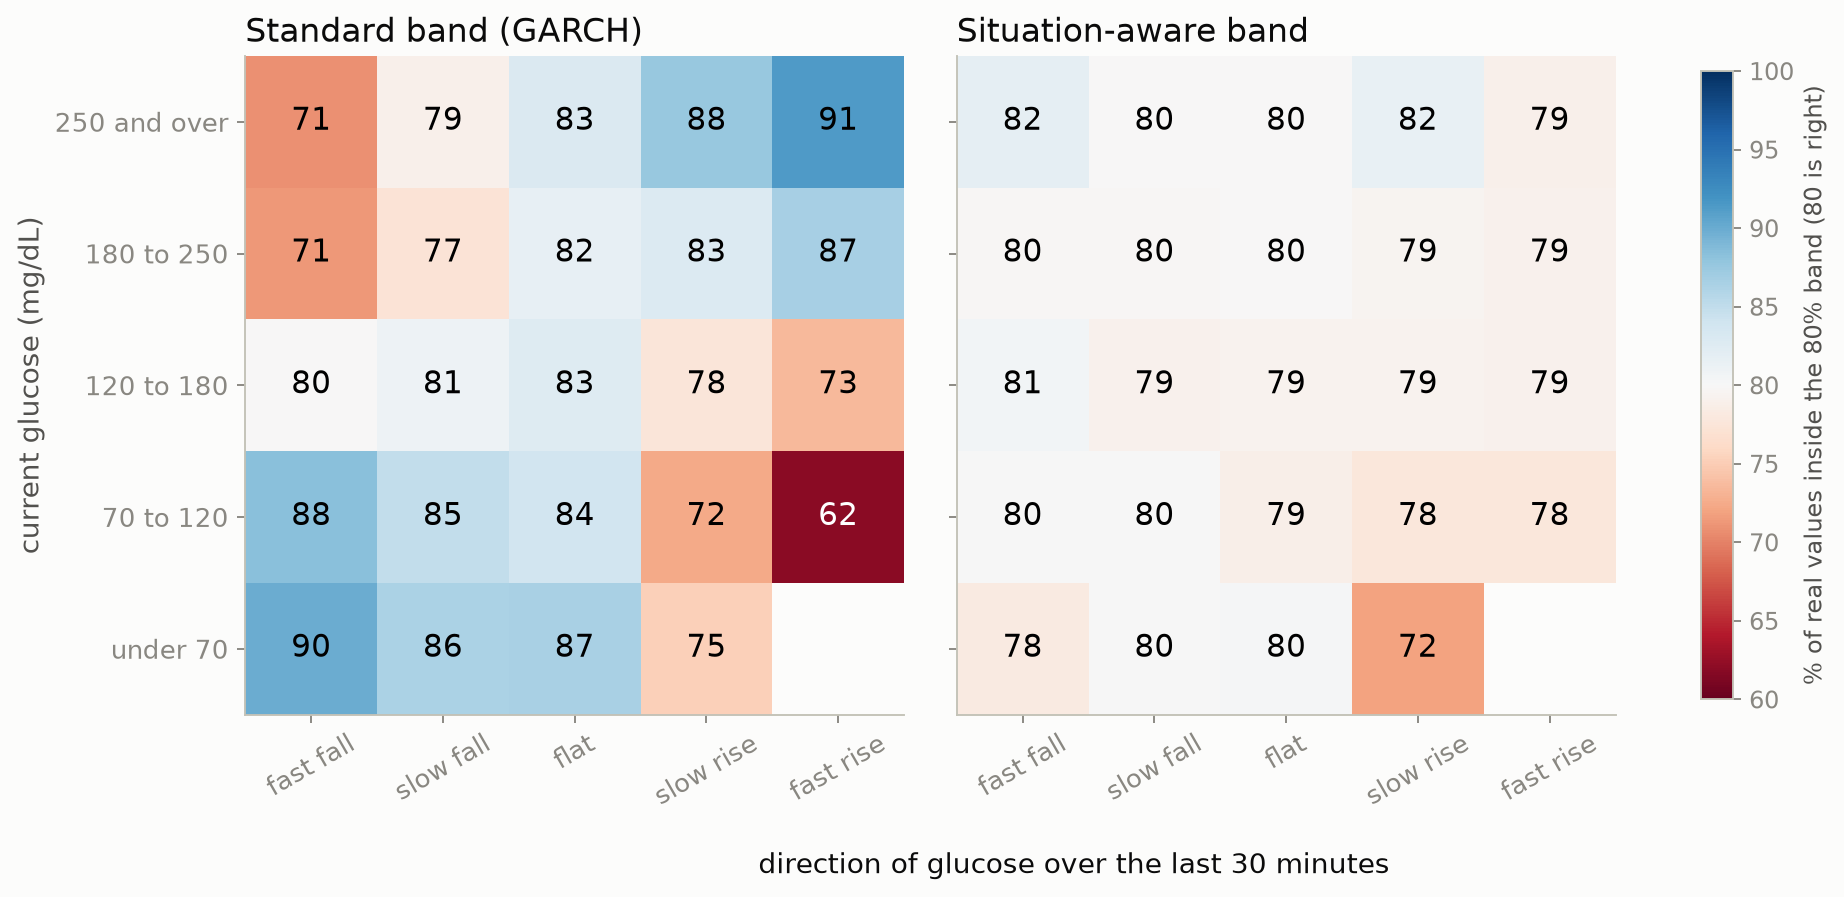
\includegraphics[width=\linewidth]{figures/situation_vs_garch.png}
\caption{Share of true glucose values inside the 80\% band in each situation, with the test forecasts of all 215 patients from the 11 datasets combined. Left: the standard GARCH band (62\% to 91\%). Right: the situation-aware band (72\% to 82\%). Rows are the current glucose level and columns the 30-minute trend; a value of 80 is on target. The empty cell (below 70 mg/dL, rising fast) had fewer than 100 test windows and is not shown.}
\label{fig:situation}
\end{figure}

\subsection{External Validation}

Because the method was designed on the three development datasets, it was then tested on the eight held-out MetaboNet datasets (153 patients). The rule for success was written down before the run: the situation-aware band had to show at least 20\% lower calibration error across situations than GARCH in at least six of the eight datasets. The rule was met in all eight datasets (Figure~\ref{fig:external}). The situation-aware band was 2.3 to 4.2 percentage points from 80\% on average, against 5.5 to 6.8 points for GARCH, a reduction of between 29\% and 67\% depending on the dataset. Overall coverage stayed close to the target (78.5\% to 81.2\%), and the bands were narrower than GARCH in every dataset, by about 8 to 12 mg/dL in average full width (84 to 99 mg/dL against 94 to 108 mg/dL).

\begin{figure}[htbp]
\centering
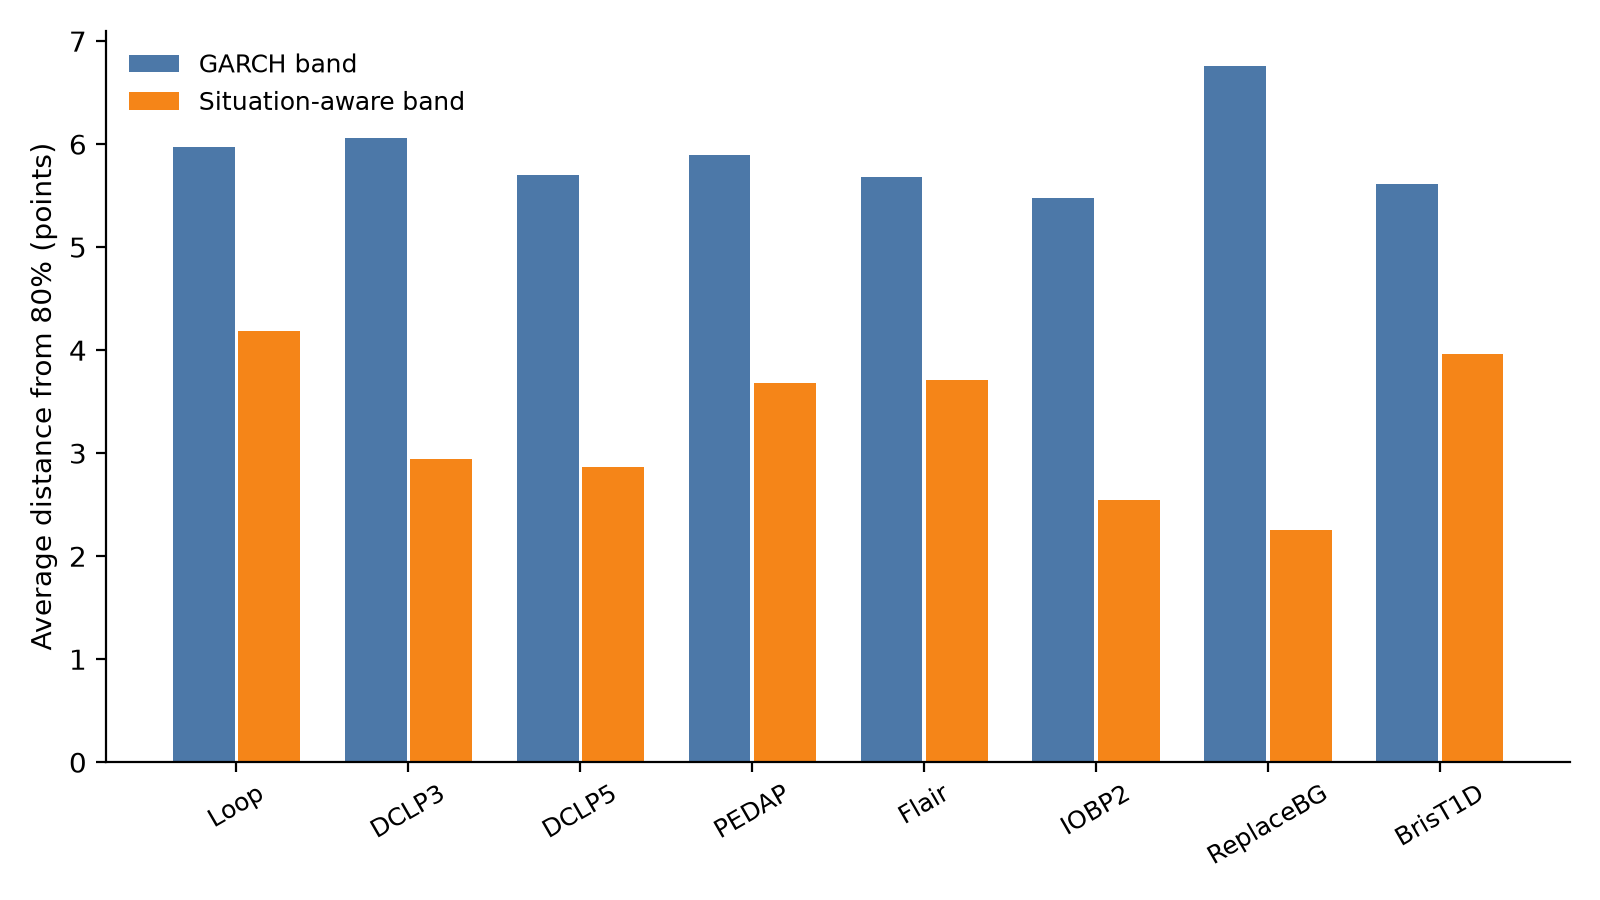
\includegraphics[width=0.8\linewidth]{figures/external_situation_distance.png}
\caption{External validation on the eight held-out MetaboNet datasets (13 to 20 patients each): average distance from 80\% coverage across situations, in percentage points, for the GARCH band and the situation-aware band. Lower is better.}
\label{fig:external}
\end{figure}

\section{Discussion}
\label{sec:discussion}

The initial result suggests that a band can be honest on average while being systematically too narrow or too wide in specific situations, and that sizing the band by situation removes most of this unevenness without widening it. Because the gain held on eight datasets never used to design the method, it is less likely to reflect tuning to the development data. The main limitation is that a band that is honest in every situation does not necessarily catch more dangerous forecast errors: consistency is a property of honesty, not of clinical benefit.

\section{Data Availability}
\label{sec:availability}

AZT1D \parencite{azt1d2025} and HUPA-UCM \parencite{hupa2024} were downloaded from Mendeley Data and are released under the Creative Commons Attribution 4.0 (CC BY 4.0) license. OhioT1DM and the eight held-out datasets were taken from the public MetaboNet file \parencite{metabonet2026}. The consolidated MetaboNet file is licensed for non-commercial research and educational use, and its component datasets keep their original licenses: those hosted by the Jaeb Center for Health Research follow the Jaeb terms of use, and the others are under CC BY 4.0 \parencite{metabonetbench2026}. The code for this paper is available at \url{https://github.com/TomerWeissman/capstone}.
